%!TEX root = volumeFinal.tex 
\chapter{Planejamento}
\label{chap:planejamento}

As pessoas realizam a atividade de planejar alguma coisa muitas vezes por dia.
Algumas vezes esse planejamento é muito simples, como organizar as tarefas que serão feitas no próximo dia, outras vezes pode ser mais complexa como organizar uma viagem de final de ano. Planejar implica em elaborar uma sequência de ações com o intuito de alcançar um objetivo, ou seja, o processo de planejar consiste em organizar as ações, antecipando os resultados esperados de cada ação para conquistar um objetivo. 

O planejamento na área da IA é uma subárea de estudo que se usa para encontrar um plano que resolva um problema específico. Como os ambientes nem sempre possuem as mesmas características, existem diferentes técnicas que são usadas para construir um plano.

\section{Planejamento automatizado}
\label{sec:classicalPlanning}

Planejamento automatizado estuda o processo de geração de planos computacionalmente. O objetivo do planejamento é encontrar uma sequência de ações que solucione um problema, a sequência de ações encontrada é chamada de plano. Para construir um plano é utilizado um planejador. O planejador recebe uma descrição formal de um problema de planejamento e tenta solucionar esse problema, para isto podem ser utilizados algoritmos de buscas e heurísticas~\cite{ghallab2004automated}\cite[Capítulo 10]{intelligence2003modern}.

\subsection{Representação de um problema de planejamento}
\label{subsec:classicalPlanningRep}

Uma das maneiras de representar um problema de planejamento é utilizando lógica proposicional.
A lógica proposicional é expressa através de sentenças atômicas, que são compostas de proposições. 
Cada proposição pode assumir um valor verdadeiro ou falso. 
Por exemplo, para representar que uma lâmpada está apagada, pode ser utilizado a proposição $apagada$.
Se a lâmpada estiver apagada, a proposição assume o valor verdadeiro. 
Junto com as proposições podem ser usados conectivos lógicos como negação (\textit{not}) $\neg$, conjunção (\textit{and}) $\wedge$ e disjunção (\textit{or}) $\vee$. 
No exemplo da lâmpada, pode-se representar que a luz está apagada e a TV está ligada, uma forma de fazer isto é $apagada~ \wedge~ ligada$. 
A lógica proposicional pode ser considerada simples mas serve de base para as lógicas mais expressivas~\cite[Capítulo 10]{intelligence2003modern}. 

Como a lógica proposicional tem expressividade limitada, é preciso utilizar uma lógica que consiga expressar mais sobre os estados do ambiente que desejamos representar. 
A lógica de primeira ordem (LPO) estende a lógica proposicional e diferentemente da lógica proposicional consegue representar relação entre preposições, ou seja, as preposições podem ter aridade maior que um, um exemplo pode ser um objeto estar sobre o outro ($sobre(A,B)$). Outra diferença da LPO é a possibilidade de utilizar quantificadores para demonstrar fatos comuns sobre as preposições, como objetos que tenham a mesma cor ($\forall x~ azul(x)$).

A descrição formal de sentenças em LPO é composta por um predicado seguido de uma lista de termos, denotada por $p(t_{0}, t_{1}, ..., t_{n})$. 
Um predicado se refere a uma relação existente entre os termos, que são objetos que se referem a objetos definidos, indefinidos ou a funções \cite[Capítulo 10]{intelligence2003modern}. 
No exemplo da lâmpada, pode-se dizer que a lâmpada da cozinha está apagada, pelo predicado $apagada(cozinha)$. 
Ou ainda, que a lâmpada do quarto está apagada e a TV da sala está ligada, $apagada(quarto)~ \wedge~ ligada(sala)$.  

\subsection{Formalização de um problema de planejamento}
\label{subsec:classicalPlanningForm}

Alguns conceitos são importantes para entender a formalização de um problema de planejamento. 
Os estados são um conjunto de átomos que não podem ser divididos em sub fórmulas, eles assumem valores de verdadeiro ou falso dependendo da interpretação do ambiente.
As ações alteram o estado do ambiente e para que sejam aplicadas é preciso que um conjunto de precondições seja satisfeito.
Se for, é aplicado um conjunto de efeitos sobre o ambiente~\cite[Capítulo 10]{intelligence2003modern}.
Por exemplo, mover um objeto de um lugar para o outro é preciso um predicado que defina que um objeto está em determinado lugar. Esse exemplo é representado abaixo:

\begin{itemize}
	\item Ação: $move(from, to)$
	\item Precondição: $at(from)$
	\item Efeito: $\neg at(from) \wedge at(to)$
\end{itemize}

Uma ação $a$ é aplicável em um estado $s$ se todas as precondições do estado $s$ forem satisfeitas, o resultado gerado pela execução de $a$ no estado $s$ é um novo estado $s'$.
Nele são aplicados todos os efeitos, removendo os predicados negativos e adicionando os positivos~\cite{meneguzzi2015planning}.

Os operadores são definidos como $op = (nome(t), precond(p), efeitos(p)$. 
O $nome(t)$ é o nome do operador e $t$ é o conjunto de termos que compõem as precondições e os efeitos. $precond(p)$ é o conjunto de predicados que representam as precondições do operador. $efeitos(p)$ é o conjunto de predicados que serão aplicados ao ambiente após a execução do operador.
Todos os operadores disponíveis para a resolução do problema formam a descrição das ações~\cite{ghallab2004automated}.
 
Como nas técnicas de busca, em planejamento também é necessário ter uma descrição do problema.
Formalmente, um problema de planejamento pode ser descrito como $P = (\Sigma, s_{0}, g)$, onde $\Sigma$ é o domínio, onde consta a descrição do problema com as ações disponíveis, $s_{0}$ é o estado inicial onde o problema começa e $g$ é o objetivo~\cite{ghallab2004automated}. 
Voltando ao exemplo do Capítulo~\ref{chap:busca}, onde um agente tenta chegar a cidade de Porto Alegre partindo da cidade de São Jerônimo e as ligações entre as cidades são caminhos que o agente pode transitar, podemos formalizá-lo como:

\begin{itemize}
	\item \textbf{estado inicial} ($s_{0}$) = $At(S$\~a$o~Jer$\^o$nimo)$;
	\item \textbf{objetivo} ($g$) = $At(Porto~Alegre)$; e
	\item \textbf{domínio} ($\Sigma$) = 
	\begin{itemize}
		\item nome: $move(cityA, cityB)$
		\item precondições: $at(cityA) \wedge link(cityA, cityB)$
		\item efeitos: $\neg at(cityA)~ \wedge at(cityB)$.
	\end{itemize}
\end{itemize}

O processo de geração do plano é feito pelo planejador. 
Um plano é uma sequência de operadores gerada a partir de um problema que, quando executada partindo do estado inicial, modifica o estado de forma que o objetivo seja válido no estado resultante. 
A Figura~\ref{fig:planmodelo} ilustra o comportamento do planejador.

\begin{figure}[ht]
	\centering
	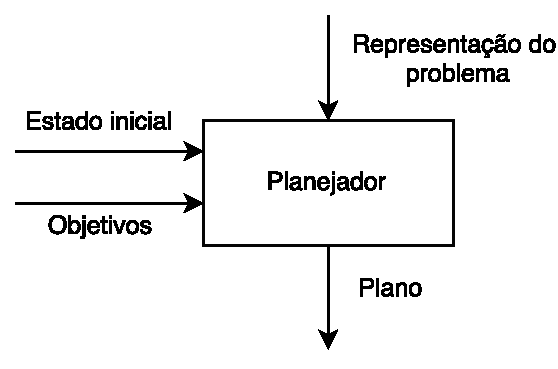
\includegraphics[width=0.4\textwidth]{fig/modelo.pdf}
	\caption{Problema de planejamento clássico.}
	\label{fig:planmodelo}
\end{figure} 

Um plano é considerado ótimo quando não há nenhum outro plano que atinga o objetivo utilizando um menor custo das ações que ele.
Uma forma de gerar planos ótimos é utilizando técnicas de busca combinadas com alguma heurística que seja independente de domínio.
Uma heurística deve ser computacionalmente eficiente e ter precisão para que a geração do plano seja eficiente~\cite{helmert2007flexible}.

\section{Planejamento hierárquico} 
\label{sec:htnPlanning}

O planejamento clássico consegue gerar planos ótimos.
Mas o tratamento de problemas de grande complexidade pode se tornar intratável.
Isso acontece por conta do poder computacional necessário para que o plano consiga ser gerado.
O planejamento clássico possui uma expressividade limitada, pois não é possível representar quando uma ação irá ocorrer, por exemplo~\cite[Capítulo 11]{intelligence2003modern}.
Como alternativa para esses problemas foi proposto o planejamento hierárquico, chamado de \textit{Hierarchical Task Network} (HTN). 
O planejamento HTN se diferencia do planejamento clássico na forma como os planos são gerados~\cite{ghallab2004automated}. 
Enquanto no planejamento clássico é necessário ter heurísticas para a geração de planos, em planejamento HTN é possível expressar conhecimento de domínio junto com os operadores, isso faz com que as ações sejam tratadas em alto nível.  
O conhecimento de domínio contém informações que determinam o espaço de estados possíveis para determinado ambiente. 
O planejador utiliza o conhecimento de domínio para percorrer os estados e encontrar os planos possíveis. 
Para isso, o conhecimento de domínio deve conter informações relativas as ações disponíveis no ambiente e as possíveis transições de estados~\cite[Capítulo 11]{intelligence2003modern}.

O objetivo do planejamento HTN é produzir uma sequência de ações que executem determinada tarefa $t$, esta tarefa está completa quando todas as tarefas não primitivas são decompostas em tarefas menores até só restarem tarefas primitivas.  
As tarefas primitivas são análogas as ações executáveis em planejamento clássico, e expressam uma atividade que o agente possa executar diretamente no ambiente~\cite[Capítulo 11]{intelligence2003modern}. 
Já as tarefas não primitivas representam objetivos que o agente deve alcançar com o intuito de decompor as tarefas não primitivas em primitivas. 
O exemplo da seção anterior, mover um objeto de lugar, é um exemplo de tarefa primitiva, pois altera o estado do ambiente, podendo ser representado em HTN como: \texttt{(move~ ?from~ ?to)}. 
Um exemplo de tarefa não primitiva é realizar uma viagem de carro, para completar essa tarefa é necessário fazer a revisão do carro, arrumar as malas e colocar as bagagens dentro do carro, uma representação destas tarefas pode ser: \texttt{(travelByCar ~?car~ ?stuffs)}. 

Para iniciar a geração de um plano HTN, deve ser usado como início uma tarefa de ligação. 
Uma tarefa de ligação HTN é definida como $w = (T, C)$, onde $T$ é um conjunto de tarefas a ser completadas e $C$ é um conjunto com relação de ordem de restrições sobre as tarefas $T$. 
As restrições estabelecem a ordem com que as tarefas $T$ devem ser executadas. 

Um domínio de planejamento HTN é um par $D = (A, M)$, onde $A$ é um conjunto de predicados que representam estados no ambiente e $M$ é o objetivo do agente expresso por um ou mais métodos do domínio~\cite{meneguzzi2015planning}. 
Um método é utilizado para decompor tarefas não-primitivas em primitivas. 
Um método é representado por $m = (p, t, w)$, onde $p$ é uma precondição que estabelece o que deve estar presente no estado atual para que a tarefa $t$ consiga ser decomposta por uma tarefa de ligação $w$~\cite{ghallab2004automated}. 
Considerando o exemplo anterior de viajar de carro, a Figura~\ref{fig:htnmethod} ilustra esse método, sendo a tarefa em cinza uma tarefa não primitiva, que posteriormente também será decomposta. 
O losangolo representa as precondições, as sub tarefas representam o conjunto de tarefas que faz parte da tarefa de ligação, e a ordem das sub tarefas caracteriza as restrições. 

\begin{figure}[ht]
	\centering
	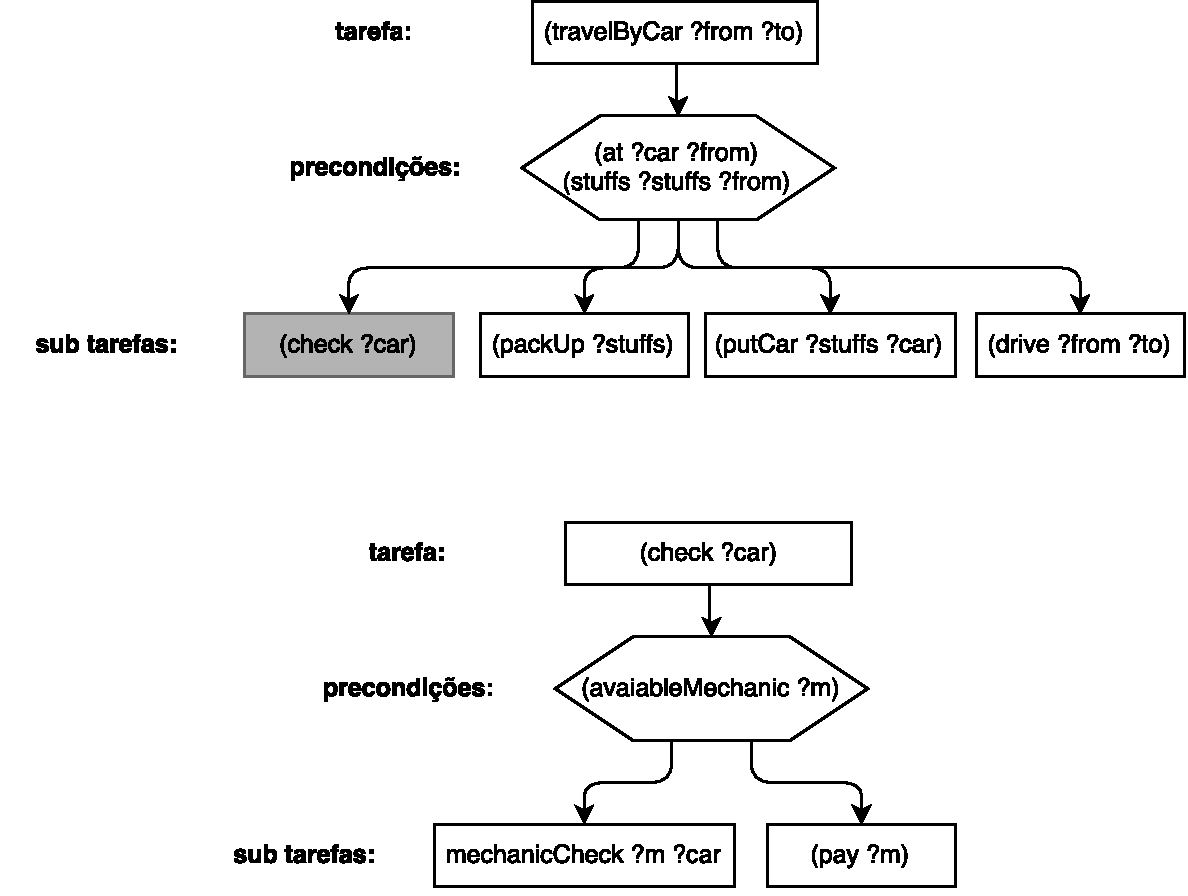
\includegraphics[width=0.7\textwidth]{fig/htnmethod.pdf}
	\caption{Exemplo de método HTN.}
	\label{fig:htnmethod}
\end{figure} 

Um problema de planejamento HTN $P$ é definido como $P = (d, I, D)$, onde $D$ é um domínio, $d$ é a tarefa de ligação inicial e $I$ é um estado inicial como no planejamento clássico. 
O processo de geração de um plano utilizando planejamento HTN consiste em encontrar um método que consiga ser aplicado na primeira tarefa de $d$, isso faz com que seja gerada uma tarefa de ligação diferente $d'$, onde a primeira tarefa foi decomposta. 
Esse processo continua, agora aplicado a $d'$, até que todas as tarefas sejam primitivas \cite{meneguzzi2015planning}. 
Se em algum ponto, nenhum método consiga ser aplicado, o planejador deve realizar um retrocesso (\textit{backtracking}), que consiste em voltar a um $d$ anterior a ponto de conseguir aplicar outra decomposição \cite[Capítulo 11]{intelligence2003modern}. 
É possível representar a busca do plano por uma árvore $N$, na qual os nodos são tarefas ou métodos. 
Cada tarefa não-primitiva pode ter apenas um filho, que deve ser um método. 
Cada método deve ter um filho para cada uma das suas sub tarefas. 
Tarefas primitivas não podem ter filhos, o que significa que elas não podem ser decompostas. 
Uma árvore totalmente decomposta é onde todas as folhas de $N$ são tarefas primitivas \cite{ontanon2015adversarial}. 
A Figura~\ref{fig:htnmethodtree} ilustra a árvore de resolução do exemplo anterior.

\begin{figure}[ht]
	\centering
	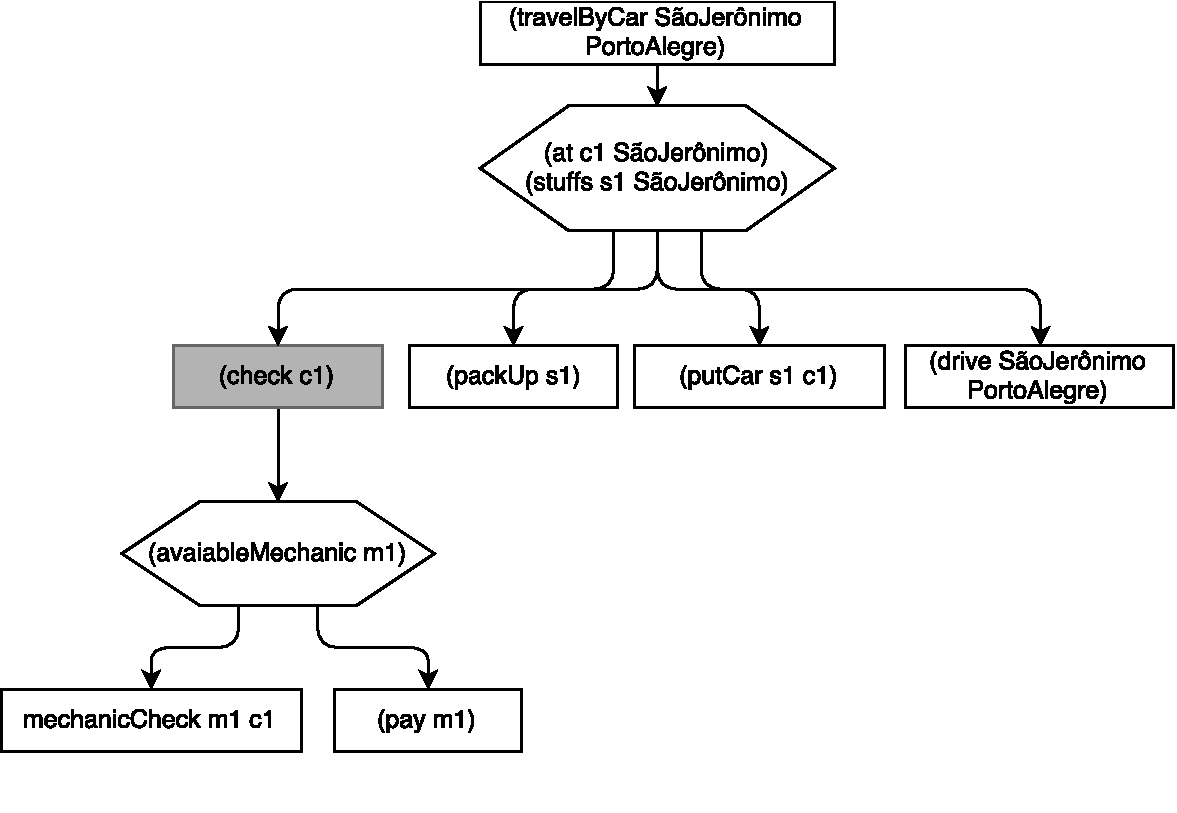
\includegraphics[width=0.7\textwidth]{fig/htnmethodresult.pdf}
	\caption{Arvore de resolução HTN.}
	\label{fig:htnmethodtree}
\end{figure}

O algoritmo de \textit{Total-order Forward Decomposition} (TFD) é utilizado para gerar um plano a partir de uma rede de tarefas inicial com ordenação total, como detalhado no Algoritmo~\ref{alg:tfd}.
O algoritmo gera as ações na mesma ordem que serão executadas, então a cada vez que uma tarefa é alcançada, tudo que antecede a mesma já foi planejado \cite{ghallab2004automated}.
 
\begin{algorithm}
	\caption{Total-order Forward Decomposition}
	\label{alg:tfd}
	\begin{algorithmic}[1]		
		\Function {TFD}{$s, <t_{1}, ...,t_{k}>, O, M$}
			\If {$k = 0$}
				\State	\Return $<>$
			\EndIf
			\If {$t_{1}$ é primitivo}
				\State $ativo = \{(a, b)~ |$ $a$ é uma instancia de $O$ e é aplicável a $s$ e b é uma substituição que torna $a$ relevante para $b(t_{1})\}$
				\If {$ativo = \emptyset$}
					\State \Return falha
				\EndIf
				\State escolhe algum par $(a, b) \in ativo$
				\State $\pi = TFD(\gamma(s, a), b(<t_{2}, ..., t_{k}>, O, M))$
				\If {$\pi = falha$}
					\State \Return falha
				\Else 
					\State \Return $a . \pi$
			\EndIf
			
			\Else
				\State $ativo = \{m |~ m$ é aplicável a $s$ e $m \in M\}$
				\If {$ativo = \emptyset$}
					\State \Return falha
				\EndIf
				\State escolhe algum par $(m, b) \in ativo$
				\State $w =~ $subtarefas$(m).b(<t_{2}, ..., t_{k}>)$
				\State \Return $TFD(s, w, O, M)$
				\EndIf
		\EndFunction
	\end{algorithmic}
\end{algorithm}

\section{Adversarial hierarchical-task network} \label{sec:ahtn}

\textit{Adversarial hierarchical-task network} (AHTN) é um algoritmo desenvolvido para lidar com o problema do grande fator de ramificação dos jogos em tempo real~\cite{ontanon2015adversarial} utilizando conhecimento de domínio no estilo de planejamento HTN. 
Nele são combinadas técnicas de HTN com o algoritmo \textit{minimax search}. 
O algoritmo assume jogos totalmente observáveis, baseados em turno e determinísticos. 

O Algoritmo~\ref{alg:ahtn}~\cite{ontanon2015adversarial} é a representação da técnica de AHTN, e assume que existem dois jogadores, \textsc{Max} e \textsc{Min}, como no algoritmo de \textit{minimax search} apresentado na Seção~\ref{sec:minimax}. 
O algoritmo também assume uma busca em árvore com uma profundidade máxima $d$. 
O intuito do algoritmo de AHTN é gerar os melhores plano para \textsc{Max} e \textsc{Min}, junto com o resultado de uma função de avaliação para quando os planos chegam a um estado terminal. 

\begin{algorithm}
	\caption{Adversarial hierarchical-task network}
	\label{alg:ahtn}
	\begin{algorithmic}[1]		
		\Function {AHTNMax}{$s, N_{+}, N_{-}, t_{+}, t_{-}, d$}
		\If {$terminal(s) \vee d \leq 0$}\label{alg:lin:firstLine}
		\State	\Return $(N_{+}, N_{-}, e(s))$
		\EndIf
		\If {$nextAction(N_{+}, t_{+}) \neq \perp$} \label{alg:ahtn:nexaction}
		\State $t = nextAction(N_{+}, t_{+})$ 
		\State \Return $\Call{AHTNMin}{(\gamma(s,t), N_{+}, N_{-}, t, t_{-}, d-1)}$ \label{alg:ahtn:troca}
		\EndIf
		\State $N_{+}^{*} = \perp, N_{-}^{*} = \perp, v^{*} = -\infty$
		\State $\aleph = decompositions_{+}(s, N_{+}, N_{-}, t_{+}, t_{-})$ \label{alg:decompositions}
		\ForAll{$N \in \aleph$} \label{alg:ahtn:for}
		\State $(N^{'}_{+}, N^{'}_{-}, v^{'}) = AHTNMax(s, N, N_{-}, t_{+}, t_{-}, d)$
		\If{$v^{'} > v^{*}$}
		\State $N_{+}^{*} = N^{'}_{+}, N_{-}^{*} = N^{'}_{-}, v^{*} = v^{'} $
		\EndIf
		\EndFor		
		\State \Return $(N_{+}^{*}, N_{-}^{*}, v^{*} )$
		\EndFunction
	\end{algorithmic}
\end{algorithm}

O algoritmo de AHTN gera uma árvore das jogadas. Cada nodo da árvore é definido por uma tupla $(s, N_{+}, N_{-}, t_{+}, t_{-})$, onde $s$ é o estado corrente do ambiente, $N_{+}$ e $N_{-}$ são a representação de planos HTN para os jogadores \textsc{Max} e \textsc{Min}, respectivamente, $t_{+}$ e $t_{-}$ representam ponteiros para qual parte do plano HTN está sendo executada, sendo $t_{+}$ para uma tarefa de $N_{+}$ e $t_{-}$ para uma tarefa de $N_{-}$. Cada nodo da árvore representa um estado do jogo~\cite{ontanon2015adversarial}.

O algoritmo alterna a perspectiva dos jogadores sempre que existir uma tarefa primitiva no plano atual, e assim avança na profundidade da árvore das jogadas. A função $AHTNMin$ é responsável pela mudança de perspectiva e ela está presente no bloco que inicia na Linha~\ref{alg:ahtn:nexaction}. No mesmo bloco há a função \texttt{nextAction(N,t)}, que é responsável por verificar se é possível a troca de perspectiva. Ela recebe como parâmetro um plano ($N$) e um ponteiro ($t$). Com isso ela retorna um ponteiro para a próxima tarefa primitiva, caso ainda não haja uma tarefa primitiva no plano, a função retorna $t = \bot$.

Caso não seja possível trocar de perspectiva, o algoritmo de AHTN decompõe o plano. O método $decompositions$ é responsável por decompor o plano atual a partir do estado do jogo na árvore. O método apenas adiciona novos planos que utilizem apenas um novo método ao plano atual. A chamada deste método ocorre na Linha~\ref{alg:decompositions} do algoritmo gerando novos planos.
O algoritmo utiliza as decomposições para comparar todos os planos gerados por uma função de avaliação. O plano que tiver a melhor função de avaliação é escolhido como melhor caminho. O plano escolhido é retornado junto com o resultado da função de avaliação. Este processo está presente na Linha~\ref{alg:ahtn:for}.

O plano pode acabar quando a profundidade limite for atingida, ou quando um estado terminal for alcançado.
Quando alguma dessas condições for alcançada, é retornado o plano das duas perspectivas e a função de avaliação para o estado do jogo atual. A Linha~\ref{alg:lin:firstLine} mostra essa condição.

A grande diferença entre o algoritmo de $AHTN$ e o algoritmo do \textit{minimax search} é que as chamadas recursivas nem sempre se alternam entre \textsc{Max} e \textsc{Min}. 
O algoritmo troca de nodos \textsc{Max} para \textsc{Min} apenas quando os planos estão totalmente decompostos a ponto de gerar uma ação (Linha \ref{alg:ahtn:troca})~\cite{ontanon2015adversarial}.

A Figura~\ref{fig:ahtn}\footnote{Figura extraída de~\cite{ontanon2015adversarial}} é utilizada para exemplificar o funcionamento do algoritmo~\ref{alg:ahtn}. 
Na raiz da árvore há apenas uma tarefa não primitiva \textit{win} para ser decomposta, para os dois jogadores. 
Há duas decomposições que o jogador \textsc{Max} pode aplicar para seu plano HTN, resultando nos nodos $n_{1}$ e $n_{5}$. A decomposição $n_{1}$ não resulta em nenhuma ação primitiva, e por isso $n_{1}$ continua um nodo \textsc{Max}. Uma vez que o jogador \textsc{Max} decompõe seus planos e há tarefas primitivas para serem executadas (nodos $n_{2}$ e $n_{5}$), é o turno de \textsc{Min} decompor suas tarefas não primitivas. Após \textsc{Min} gerar suas ações, a profundidade máxima ($d = 2$) foi atingida (nodos $n_{3}$ e $n_{4}$). 
A função de avaliação $e$ é aplicada para cada um dos estados do jogo para determinar o valor das folhas.

\begin{figure}[ht]
	\centering
	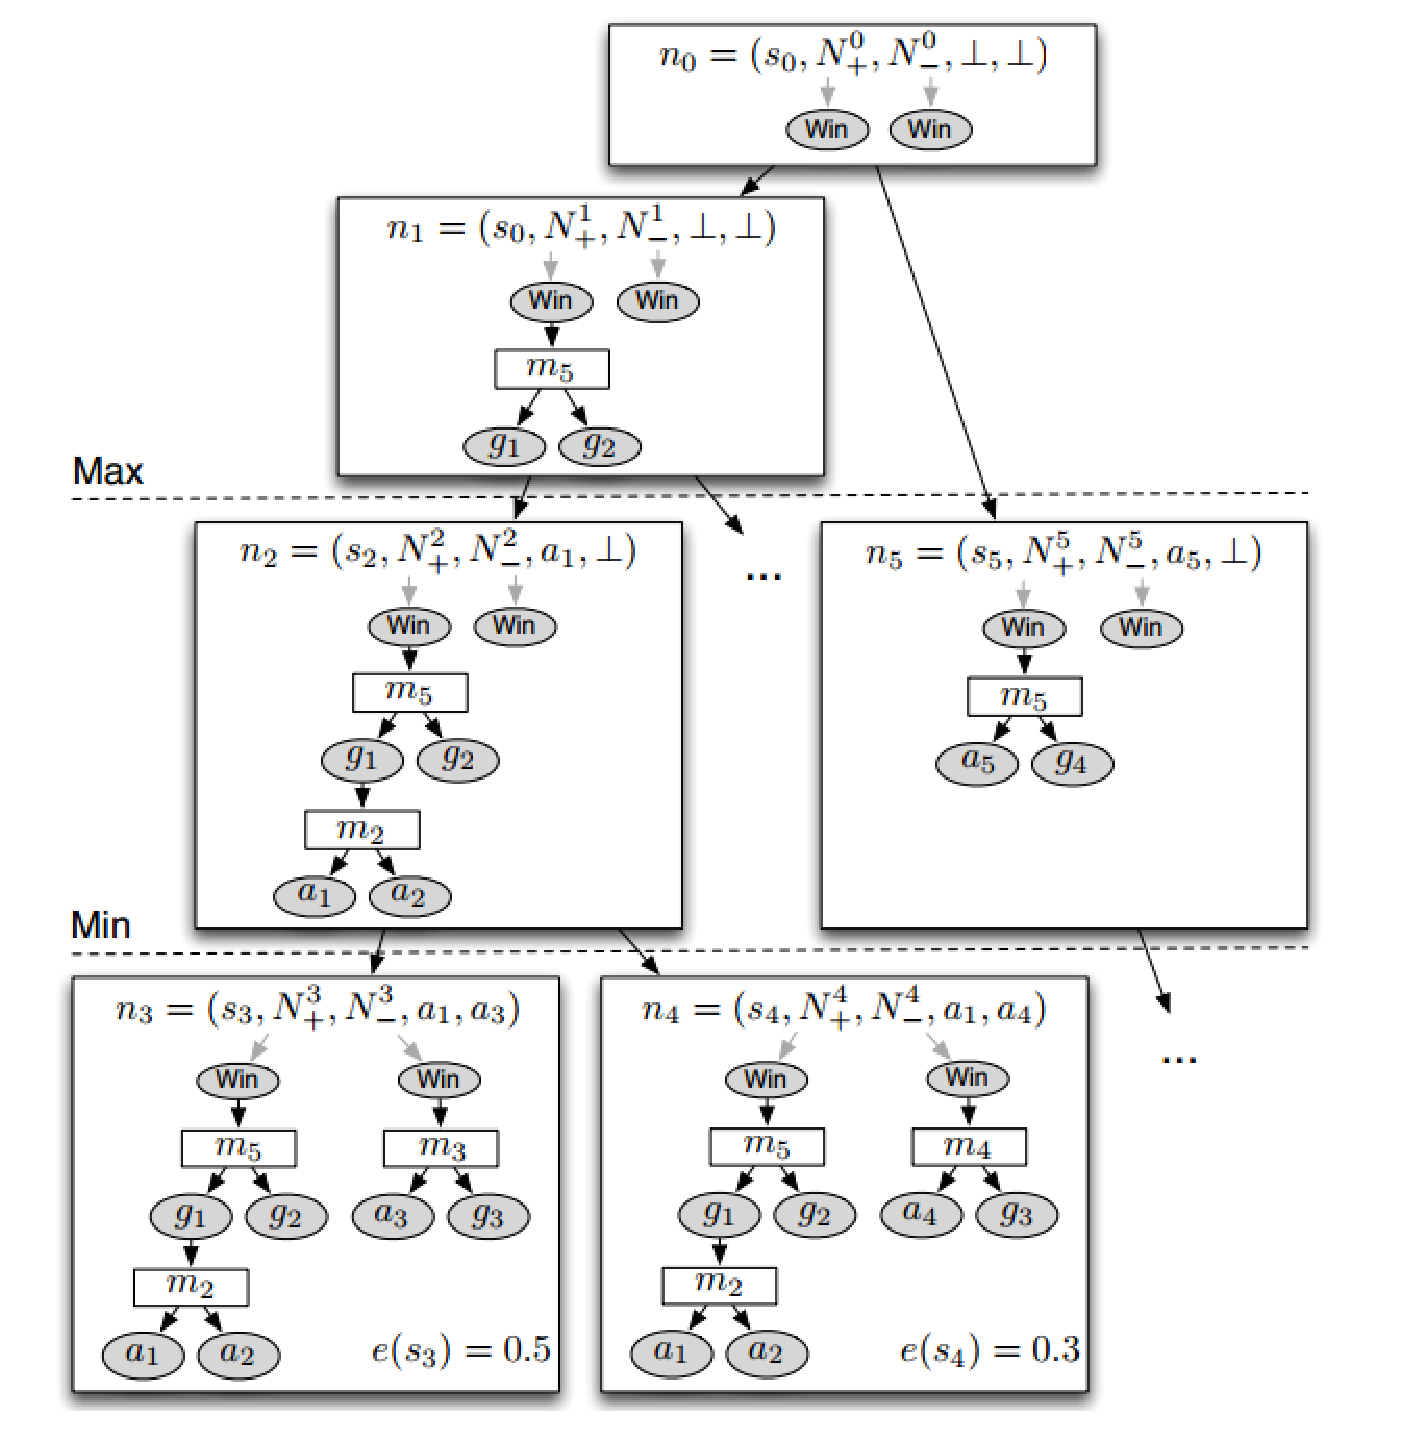
\includegraphics[width=0.8\textwidth]{fig/ahtn.pdf} 
	\caption{Árvore gerada pelo algoritmo de AHTN.}
	\label{fig:ahtn}
\end{figure}

O problema com que o algoritmo de AHTN tenta lidar é o grande fator de ramificação e o pouco tempo para determinar a próxima ação do agente. 
O algoritmo utiliza planejamento através do conhecimento de domínio para diminuir a combinação de ações que não tem nenhuma chance de serem utilizadas em determinado ambiente~\cite{ontanon2015adversarial}.
